\documentclass[a4paper]{article}

\usepackage[english]{babel}
\usepackage[utf8]{inputenc}
\usepackage{amsmath}
\usepackage{amssymb}
\usepackage{centernot}
\usepackage{graphicx}
\usepackage{listings}
\usepackage{color}
\usepackage{booktabs}
\usepackage{hyperref}
\usepackage{tcolorbox}
\hypersetup{
 colorlinks=true,
 linkcolor=blue,
 urlcolor=blue
}


\lstset{
	breaklines=true,
	basicstyle=\footnotesize,
	mathescape=false,
	frame=single,
	keepspaces=true,
	keywordstyle=\color{blue}
}


\lstdefinestyle{Bash}
{language=bash,
keywordstyle=\color{blue},
basicstyle=\ttfamily,
morekeywords={peter@kbpet},
alsoletter={:~$},
morekeywords=[2]{peter@kbpet:},
keywordstyle=[2]{\color{red}},
literate={\$}{{\textcolor{red}{\$}}}1 
         {:}{{\textcolor{red}{:}}}1
         {~}{{\textcolor{red}{\textasciitilde}}}1,
}



\usepackage{titlesec}

\setcounter{secnumdepth}{4}

\titleformat{\paragraph}
{\normalfont\normalsize\bfseries}{\theparagraph}{1em}{}
\titlespacing*{\paragraph}
{0pt}{3.25ex plus 1ex minus .2ex}{1.5ex plus .2ex}


\newcommand*{\squiggly}{\rightsquigarrow}
\newcommand{\todo}[1]{{\color{red}TODO: #1\\}}


\title{A Beginner's Notes on Phosphor}
\author{Jos\'e Cambronero}







\begin{document}
\maketitle
\begin{abstract}
This document contains my personal set of notes for building and running examples with Jonathan Bell's
Phosphor\cite{bell2014phosphor}. This should be viewed as a beginners guide (as I am writing it
as I learn to use the tool myself.) Any errors or omissions here are my own.
\end{abstract}

\section{Installation/Building}
\label{install}
We begin by cloning the \href{https://github.com/Programming-Systems-Lab/phosphor}{github repository}
for the project.

\begin{lstlisting}
$ git clone git@github.com:Programming-Systems-Lab/phosphor.git
\end{lstlisting}

Phosphor is a \href{https://maven.apache.org/}{maven} project, so to build you can call
\verb|mvn package|. As per the documentation
Phosphor has been built and tested with both versions 7/8 of Oracle's Hotspot JVM and
OpenJDK's IcedTea JVM. If you run into issues with your java version, I suggest installing
\href{http://www.jenv.be/}{jenv}, which allows you to manage multiple versions of the JVM on your
machine cleanly and transparently.

\begin{lstlisting}
$ jenv local 1.8.0.66
$ mvn package
\end{lstlisting}

You should obtain a message similar to the one in Figure~\ref{fig:phosphor-build} if your build was succesful

\begin{figure}
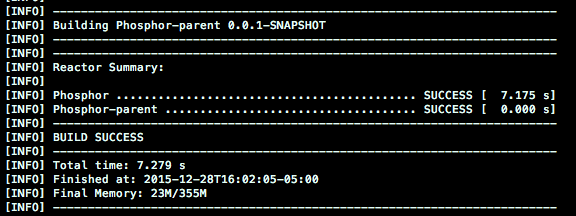
\includegraphics[width=\textwidth]{figures/phosphor-build}
\caption{Succesful build message}
\label{fig:phosphor-build}
\end{figure}

Now, we need to instrument our JRE before we can run any of our examples. This can be done
as follows

\begin{lstlisting}
$ cd target/
$ java -jar Phosphor-0.0.2-SNAPSHOT.jar \
 /Library/Java/JavaVirtualMachines/jdk1.8.0_66.jdk/Contents/Home/jre/ jre-inst/
\end{lstlisting}

This has created an instrumented JRE suitable for data flow tracking and integer
tags combined with $OR$.

The only thing left to do is make sure we change permissions for all binaries in
the instrumented JRE.

\begin{lstlisting}
$ chmod +x jre-inst/bin/*
\end{lstlisting}

\section{Testing}
In order to verify that your build works, you can run the \verb|mvn verify| command, as explained in the documentation.
You should expect this to take a bit, as it generates different instrumented JREs and tests them. If all is succesful,
you will obtain a Maven log message printed to stdout indicating so.

\section{Usage}
\subsection{Automatic}
\todo{this remains to be experimented with}
\todo{taintSinks/taintSources usage}


\subsection{Data flow}
In this section we will focus on examples that track taint from data flow operations, usually referred to as 
explicit flows\cite{denning1976lattice}. Assume $x$ is tainted, an operation such as $y = x * 2$ taints $y$.

\subsubsection{Integer taint tags}
Phosphor allows users to track taint tags represented as integers (allowing up to 32 different taint
tags), or objects, which allows up to $2^{32}$ tags. In this section we focus on integer taint tags.
Consequently, we also focus our API attention to \verb|edu.columbia.cs.psl.phosphor.runtime.Tainter|.
In it, we will primarily use 2 methods, as noted in the
original documentantion: \verb|taintedX|, which allows us to mark a primitive source as tainted, and
\verb|getTaint| which we can use to check for taint.

We show a series of simple examples using this across different datatypes. Note that the types 
can be easily replaced. Note that for each example we only show part of the relevant code,
the interested reader can check the source code associated with this guide
in \verb|java.com.josecambronero.IntegerTagExamples|.

\paragraph{Simple binary operation}
In this simple example, we create a source for the taint (variable $x$), and want to check
if there is taint flow from our source to a sink (variable $y$). In this case, $y$ is the result
of an assignment operation involving $x$, and thus should be tainted.

We can use \verb|Tainter.taintedInt| to taint $x$, and \verb|Tainter.getTaint| to check the taint
tag for $y$.

\begin{lstlisting}
// source
int x = 0;
// sink
int y = 0;
// primitive and taint tag
x = Tainter.taintedInt(x, 1);
y = x * 3;
// check sink for taint
assert (Tainter.getTaint(y) != 0);
\end{lstlisting}



\paragraph{Nullifying taint}
Note that the taint for a sink can change throughout the program. For example,
if we define $y$ in terms of a tainted $x$ and then redefine $y$ as a constant, the final $y$
is not tainted. The excerpt from \verb|IntegerTagExamples.testExample2|  below
shows this behavior.

\begin{lstlisting}
// source
int x = 0;
// sink
int y = 0;
x = Tainter.taintedInt(x, 1);
// tainted
y = x * 3;
assert (Tainter.getTaint(y) != 0);
// not tainted, as zero returns constant (not function of x)
y = zero(x);
assert (Tainter.getTaint(y) == 0);
\end{lstlisting}


\paragraph{Arithmetic identity}
Note that some arithmetic identities, which would allow a human to easily determine that no
taint exists, as the result is always constant, will yield a tainted tag with taint analysis.
So for example, in the excerpt below $y$ is tainted despite the fact that it assigned 0, regardles
of the tainted value of $x$.

\begin{lstlisting}
// source
int x = 1;
x = Tainter.taintedInt(x, 1);
// sink
int y = 0;
y = 2 * x - (x + x);
assert (Tainter.getTaint(y) != 0);
\end{lstlisting}

\paragraph{Tracking Source of Taint}
Phosphor allows the user to track the source of the taint in a sink by exploring the values
of the taint tag. A similar functionality is available for the MultiTainter by exploring
the dependencies of the tag.

In the example below, we can see that $y$ has taint stemming solely from $x$, while $z$ has
taint stemming from both $x$ and $w$, and nothing stemmed from $r$. Note that
\verb|getTaintSource| is a simple helper that checks the bits in an integer tag to find the sources,
it is not part of Phosphor.

\begin{lstlisting}
// sources
int x = 0, w = 0, r = 0;
x = Tainter.taintedInt(x, 2);
w = Tainter.taintedInt(x, 16);
r = Tainter.taintedInt(x, 4);
// sinks
int y = 0, z = 0;
y = x * 3;
z = x + w;

assert (Tainter.getTaint(y) != 0);
// get list of sources (recall taint tags are OR'ed)
List<Integer> zSources = getTaintSources(Tainter.getTaint(z));
assert (zSources.contains(Tainter.getTaint(x)));
assert (zSources.contains(Tainter.getTaint(w)));
assert (!zSources.contains(Tainter.getTaint(r)));
\end{lstlisting}

Note that we picked tag numbers that allow us to uniquely identify the sources (i.e. powers of 2),
given that the tags are combined with logical $OR$. If you need more than 32 tags, you should
look into using the MultiTaint functionality (see Section~\ref{sec:multitaint})


\paragraph{Element-level taint tags in arrays}
Phosphor maintains tags for each element in an array, rather than a tag for the
whole array\cite{bell2014phosphor}. This behavior can be seen in the excerpt below


\begin{lstlisting}
// source
int x = 0;
x = Tainter.taintedInt(x, 1);
// (potential) sinks
int[] y = new int[4];
y[0] = x * 2;
assert (Tainter.getTaint(y[0]) != 0);
assert (Tainter.getTaint(y[1]) == 0);
\end{lstlisting}



\subsection{Object taint tags}
\label{sec:multitaint}
We will now experiment with object taint tags, which allow us to create arbitrary numbers of distinct tags ($2^{32}$, which is arbitrarily large for our purposes). In order to creat object taint tags we turn to 
\verb|edu.columbia.cs.psl.phosphor.runtime.MultiTainter|, which similarly to the integer Tainter, has tainted$X$, where
$X$ is one of the various possible datatypes. As per documentation, we ignore methods
with \verb|$$PHOSPHORTAGGED| suffixes as these are for internal use.

\paragraph{Creating a simple object taint tag}
This example creates 2 tainted integers ($x$ and $y$), with two different ways of creating taint labels, and performs an addition
to create a third tainted integer $z$ (our sink). Note that we can then check the taint tag for $z$ and also print out
a string representation.

\begin{lstlisting}
// Source
int x;
x = MultiTainter.taintedInt(100, "source 1");
// Source
int y;
y = MultiTainter.taintedInt(100, new Taint("source 2"));
// Sink
int z = x + y;
Taint tz = MultiTainter.getTaint(z);
assert (tz != null);
System.out.println(tz.toString());
\end{lstlisting}

\paragraph{Creating simple object taint tags: Object variable}
Note that if we create a tainted object variable, using \verb|MultiTainter.taintedObject|, the label provided is
shown as that taint tag's label, rather than simply as a dependency. In primitives, the label is null and instead
appears in the dependency graph. Note that in contrast to the other \verb|taintedX| methods, \verb|taintedObject| has
void return. Also note that the taint tag here must be an instance of \verb|Taint|, not any object as was possible
for primitives.
\todo{Verify if this is always the case...if anyone knows better, please correct}

\begin{lstlisting}
Object s = "My string";
MultiTainter.taintedObject(s, new Taint("source x"));
Object s2 = identity(s);
Taint tag = MultiTainter.getTaint(s2);
assert (tag != null);
System.out.println((String) tag.getLabel());
System.out.println(tag.toString());
\end{lstlisting}


\paragraph{More than 32 distinct tags}
We start with a simple example that shows how we can assign more than 32 distinct tags (in this case 33).

\begin{lstlisting}
// Creating more than 32 distinct tags (the advantage of object tags)
// Array of 33 different sources
double[] mydata = new double[33];
for(int i = 0; i < mydata.length; i++) {
    mydata[i] = MultiTainter.taintedDouble((float) i, "Source " + i);
    }
    
// Sink
double result = 0.0;
for (double elem : mydata) {
    result += elem;
    }
Taint tag = MultiTainter.getTaint(result);
assert (tag != null);
System.out.println(tag.toString());
\end{lstlisting}

The print out of the tag in Figure~\ref{fig:33-tags} shows that we have 33 different taint tags as dependencies for this sink.


\begin{figure}
\includegraphics[width=\textwidth]{figures/33-tags.pdf}
\caption{We can use object tags to overcome the limit of 32 distinct taint tags with integer tags}
\label{fig:33-tags}
\end{figure}

\todo{example}
 
\paragraph{Tracing dependencies}
So far we have been simply printing out the taint tag, in which you can see the dependencies.
However, we might find it useful to actually iterate over these dependencies.
In order to do this (and to more broadly see what we can do with a Taint object),
we explore \verb|edu.columbia.cs.psl.phosphor.runtime.Taint|.
In this example, we'll use \verb|getDependencies|,
which returns a
\verb|edu.columbia.cs.psl.phosphor.struct.LinkedList|
of Taint objects.
In order to access the nodes in the linked list, you need to make sure you also import
the class \verb|edu.columbia.cs.psl.phosphor.struct.LinkedList.Node|.

\begin{lstlisting}
// Iterating over dependencies in an object taint tag
int x = MultiTainter.taintedInt(100, "x");
int y = MultiTainter.taintedInt(100, "y");
int z = x + y;
double w = MultiTainter.taintedDouble(100.0, "w");
int n = 0;

int result = z + (int) w + n;
Taint tag = MultiTainter.getTaint(result);
assert (tag != null);

LinkedList<Object> dependencies = tag.getDependencies();
System.out.println(dependencies.toString());

// iterate over the linked list
Node currNode = (Node) dependencies.getFirst();
while (currNode != null) {
    String currDepName = (String) currNode.entry;
    System.out.println(currDepName);
    currNode = currNode.next;
    }
\end{lstlisting}


\subsection{Implicit flow (control flow taints)}
\todo{experiment with implicit flows}
Note that as per Jon's explanation boolean negation becomes jump instruction so need
this section to handle things like \verb|y=!x|.

\nocite{*}
\bibliographystyle{plain}
\bibliography{biblio.bib}



\end{document}